\subsection{Physical Prototype}
\subsubsection{Use Cases}
The proposed robot does not have any intended direct applications in industry. The configuration of a planar PCR of this scale, with no ability to separate at the end effector has very little application in most contexts. It does however provide a significant use case in research of PCR control. Often PCRs that are researched intentionally have no external forces applied to their end effectors, they are operating in free space \cite{survey}. In this free configuration, the only force that control and estimation models must account for is gravity, which is related to the robot's mass. In the proposed setup, a friction force is applied to the end effector, which is related to the robot's velocity. For this component to be modelled and accounted for, researchers will be required to leave behind the semi-static assumption during modelling. The proposed platform thus provides an opportunity to expand PCR modelling in research to include a time component. 


\subsubsection{Robot Configurations}
The robot is designed both in software and hardware to accommodate changing robot configurations without a large hassle. The arm's bases are mounted on a rail that can easily be translated along any axis that the rails are fastened in. For the setup discussed in this thesis, the bases can be moved along the y-axis. Additionally, the software and control loop supports the addition of arms. A third arm could be added for example to try and gain an angular degree of freedom with the end effector. In Figure \ref{fig:workspace_simulated}, several possible workspace configurations with just the current setup are shown. Each would take less than a minute to change to. The addition of more arms can only shrink the usable workspace. The controllers presented can easily be adjusted to account for additional arms as well. The PID controller requires no modification while the differential CC controller would required the left inverse be taken in \eqref{eq:cc_diff/ik}. 

\begin{figure}[h]
    \centering
    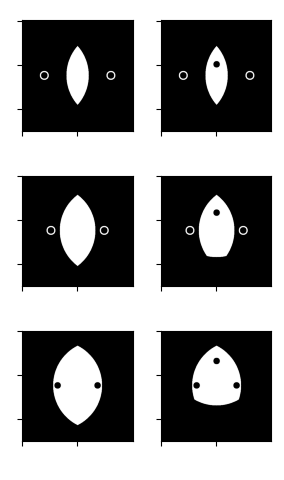
\includegraphics[width=0.4\textwidth]{images/workspaces.png}
    \caption{Simulated robot workspace with two (left) and three (right) arms in varying planar configurations}
    \label{fig:workspace_simulated}
\end{figure}

The addition of one or multiple arms can add complexity of control by allowing the user to apply arbitrary forces at the end effector at the expense of limiting the robot's workspace. A hypothetical configuration could see four arms operating; two that are used to control the robot and two that apply arbitrary end effector forces. Because of the tilting end effector issue mentioned in \ref{sec:physical_description}, the physical limitation of the current end effector is likely around four arms without a redesign.


\subsubsection{Limitations}
\label{sec:prototype_limitations_discussion}
\paragraph{Tendon slack} arises on each arm due to manufacturing inconsistencies during the tendon tensioning process. To ensure the tendon stays routed the right way, four \SI{0.75}{"} nuts are placed on it to act as a tensioning weight (Figure \ref{fig:tendon_slack}). This slight amount of slack results in an operational "dead zone" between arm contraction and extension where the robot can actuate the motors with no resulting motion in the end effector. The idea of training learning-based models that have a tunable configuration parameter comes from this effect, as the robot will have a slightly different response to control inputs in this region between tendon installations. 

\paragraph{Physical failures} coming from 3D printed parts failing is a reality of ensuring this design is reproducible for third parties. Replacement parts machined out of stronger materials could greatly improve the lifespan of the robot but are far less accessible. This trade off is a reality of this design that results in limited consistency of the robot. This may make the platform unsuitable to some research applications. 